\documentclass[a4paper,french,twoside,openright]{report}
\usepackage[utf8]{inputenc}
\usepackage[french]{babel}

\usepackage{a4wide}
\usepackage{pdfpages}
\usepackage{varioref}
\usepackage[pdftex]{hyperref}
\usepackage{cite}

\usepackage{fancyhdr}
\usepackage{array}
\usepackage{multirow}
\usepackage{longtable}
\usepackage{slashbox}
\usepackage{rotating}
\usepackage{float}
\usepackage{color}
\usepackage{colortbl}

\usepackage{graphicx}
\usepackage{epic}
\usepackage{wrapfig}
\usepackage{subfigure}

\usepackage{amsmath}
\usepackage{amsfonts}
\usepackage{mathrsfs}
\usepackage{amssymb}
\usepackage{amsthm}
\usepackage{tabularx}

\usepackage{eurosym}

\usepackage[nottoc, notlof, notlot]{tocbibind}

\DeclareGraphicsExtensions{.jpg,.mps,.pdf,.png,.gif}


\renewcommand{\headrulewidth}{0pt}
\renewcommand{\footrulewidth}{0pt}
\fancyhead{}
\fancyhead[LO,LE]{$1^\textrm{ère}$  année ENSGTI}
\fancyhead[RE]{Projet professionnel}
\fancyhead[RO]{\leftmark}


%---------- COMMANDES PERSOS
\newcommand{\unit}[1]{{\,\mathrm{#1}}}
\newcommand{\ve}[1]{{\Vec{#1}}}
\newcommand{\ma}[1]{{\mathbf#1}}
\newcommand{\nom}[1]{{\scshape#1}}
\renewcommand{\d}{{\mathrm{d}{}}}

\def \dpar #1#2 {\frac{\partial #1}{\partial #2}} 
\def \ddrt #1#2 {\frac{d #1}{d #2}} 
\def \croch #1 { \left[ #1 \right] } 
\def \paren #1 { \left( #1 \right) } 
\def \accog #1 { \left\{ #1 \right. } 

\setlongtables 

\begin{document}

\setlength{\parindent}{0mm}

\pagenumbering{roman}

\pdfbookmark[0]{Page de garde}{garde}

\begin{titlepage}
	\begin{center}
		
\includegraphics[scale=1]{photo/ensgti.jpg} 
	\end{center}
	
	\vspace*{\stretch{1}}	
	\begin{center}
		\rule[1em]{0.9\textwidth}{1mm}
		\Huge\scshape\bfseries
		\textcolor{blue}{Projet de conception}
		\\
		\textcolor{red}{Dimensionnement d'une unité de stockage de chaleur sensible}\\
		\rule{0.9\textwidth}{1mm}

	\end{center}
	\begin{center}
		\vspace{2.5cm}
		{\Large \'Energétique 2$^{\textrm{ère}}$ année}\\
		\vspace{2cm}
		{\large Promotion 2014}
		\vspace{1cm}
		\\
		{\large Pamo Charlotte, Tarroux Frédéric, Delacroix Damien}
	\end{center}
	
	\vspace*{\stretch{3}}
	{\small Fichier : \texttt{\jobname.tex}
	\hfill
	%<<Made with \LaTeX !>>
	\hfill
	Version du : \texttt{\number\day/\number\month/\number\year} }
\end{titlepage}

\pagestyle{fancy}
\renewcommand{\chaptermark}[1]{\markboth{#1}{}}

\tableofcontents
\listoffigures
\listoftables

\pagenumbering{arabic}




%PLAN
\chapter{Le stockage d'énergie par air comprimé}

\section{Introduction}

Afin de conserver l'énergie électrique non utilisée en heure creuse, le stockage par air comprimé est une solution envisageable. Actuellement, il existe deux systèmes en fonctionnement, un à Huntorf en Allemagne et l'autre à Mcintosh Alabama aux États-Unis.\\

La démarche global consiste à utiliser l'électricité pour activer des compresseurs qui comprimerons l'air ambiant pour ensuite le stocker dans une cave en sous-sol. Il y a alors transformation de l'énergie électrique en énergie mécanique. Cependant, lors de cette compression, il y a échauffement de l'air. Hors, cette énergie est perdue vers le milieu extérieur. L'objectif est donc de récupérer celle-ci grâce à un stockage de chaleur sensible. Par conséquent, nous allons dimensionner ce stockage pour la centrale de Huntorf. \\

Dans un premier temps, nous allons décrire le système. Puis nous ferons un rapide bilan thermodynamique pour vérifier si le stockage de chaleur sensible possède un intérêt. Enfin, nous réaliserons une petite analyse économique afin de quantifier les gains possibles et donc l'investissement réalisable pour construire cette installation.
\newpage

\section{Description du principe général}

\subsection{Le cycle de l'air}

\begin{figure}[!h]
\centering

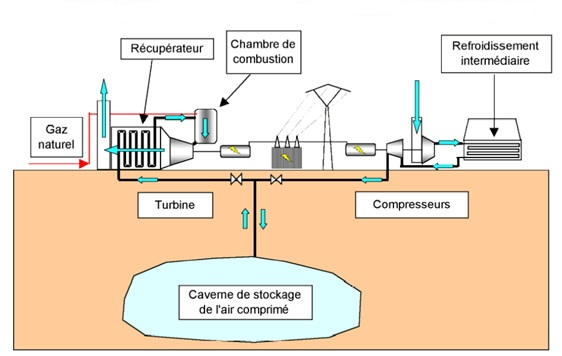
\includegraphics[scale=0.7]{PHOTO/shema_base.jpg}
\label{sh_base}
\caption{Schéma d'un stockage d'énergie par air comprimé}
\end{figure}

Comme nous pouvons le visualiser sur la figure \ref{sh_base}, l'air est comprimé par un compresseur en heure creuse. Lors de cette étape, l'air va être fortement réchauffé. Il va donc être refroidis par un échangeur classique. Ainsi fait, il va être stocké dans une caverne naturelle sous haute pression.\\


Lorsque l'on va passer en heure pleine, il va être déstocké et réchauffé par du gaz naturelle dans une chambre à combustion, notamment pour éviter que l'eau contenue dans l'air ne se condense. Cette étape est crucial puisque l'air va ensuite être détendu dans une turbine. Dans ces circonstances, il faut empêcher tous risques de cavitation, et donc d'eau sous forme liquide, pour éviter une usure prématuré de la turbine. Pour finir le cycle, la rotation de la turbine, relié à un alternateur, va produire de l'énergie sous forme électrique. Ainsi, celle ci va pouvoir être distribuée par le réseau électrique.\\


Comme nous souhaitons récupérer l'énergie perdue lors de la compression, nous allons regarder plus en détail le système "compresseur".

\subsection{La compression}
 
 Sur la figure \ref{sh_fonc}, nous remarquons la présence de trois compresseurs : basse, moyenne et haute pression. 
 
Les étages de compressions sont réalisés pour deux raisons. La plus importante est que la compression de l'air entraine une augmentation de la température du gaz. Hors, la dilatation des matériaux, provoquée par la chaleur, peut entrainer la destruction du compresseur. La solution consiste donc à refroidir les gaz, par un échangeur, entre plusieurs étages de compressions. 

L'autre raison est qu'il existe plusieurs technologies de compresseurs ce qui a pour conséquence d'avoir des coûts et rendements différents. Nous allons décrire rapidement les trois types de compresseurs utilisés dans le stockage d'air comprimé.

\subsubsection{Compresseur piston}

Le principe est relativement simple. Un piston est mis en mouvement pour comprimé l'air. Il existe des systèmes qui permettent de comprimer l'air au-dessus et en-dessous du piston. L'on peut ensuite aligner plusieurs cylindres pour atteindre de très hautes pressions.

Ces pistons permettent de d'augmenter la pressions entre 1.5 et 414 bar pour un travaille fourni comprit entre 0.75kW et 420kW.
 
\subsubsection{Compresseur à vis}

 C'est le système le plus utilisé. Chaque éléments possèdent un rotor mâle et femelle se déplacent l'un dans l'autre, provoquant ainsi une diminution du volume et donc une augmentation de pression.  
 
Il produit une élévation de pression de 5 à 13 bar pour un travaille comprit entre 4kW et 250kW.

\subsubsection{compresseur à palettes}
 
 Un rotor, possédant un certains nombres de fentes, est mis en rotation. Dans chaque fentes est inséré une palette qui par force centrifuge se déplace vers les parois provoquant ainsi la compression du gaz. La chaleur dégagé lors de la compression est contrôlé par injection d'huile.
 
 Ces pistons permettent de d'augmenter la pressions de 7 à 10 bar pour un travaille fourni comprit entre 1.1kW et 75kW.\\
 
 Ayant étudié le système, nous allons estimer la chaleur perdu par compression et la chaleur fournie par combustion.
 
\section{Calcule de l'énergie perdue et nécessaire par le système}

Il est estimé que si l'on pouvais récupérer la chaleur dégagé lors de la compression, l'on pourrai réduire la consommation de gaz naturel de 25\%. Pour l'usine de Huntorf, 5600kJ de gaz naturel pour 1Kwh d'énergie en sortie est nécessaire. L'objectif de cette partie va être de comparer la chaleur produite par compression et par combustion pour vérifier si il est pertinent de dimensionner un stockage de chaleur sensible.


\subsection{Calcule de la chaleur perdue}

Nous allons estimer, par les principes thermodynamiques, la chaleur dégagée par la compression. 

Celui ci est établie à partir des données visualisables sur la figure \ref{sh_fonc} et du tableau \ref{tab1}.\\


\begin{figure}[!h]
\centering
\caption{Schéma de la centrale de Mcintosh avec certaines grandeurs thermos-physiques}
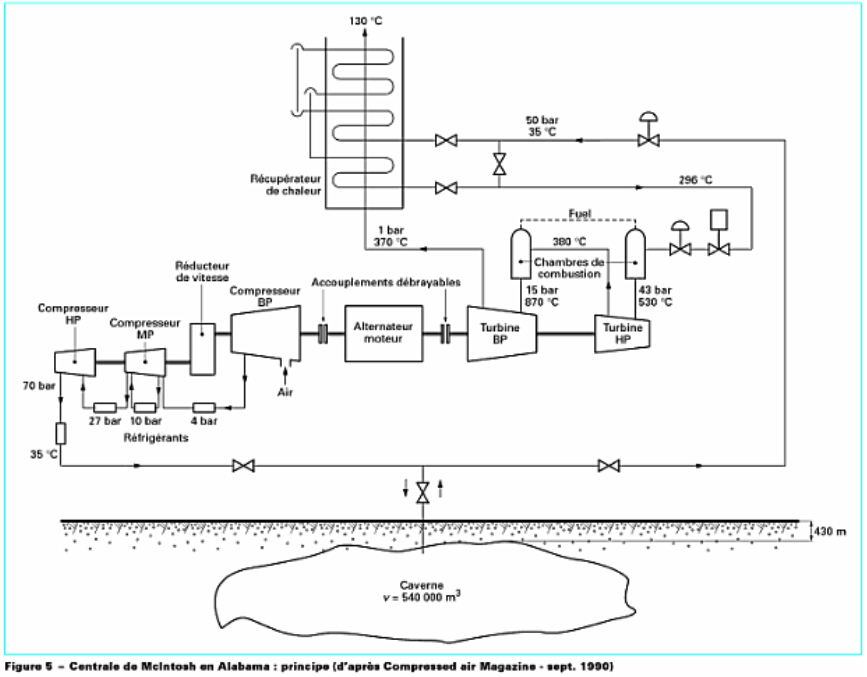
\includegraphics[scale=0.5]{PHOTO/shema_fonctionnement.jpg}
\label{sh_fonc}
\end{figure}


\begin{figure}[!h]
\centering
\caption{Tableau regroupant certaines données de la centrale de Huntorf}
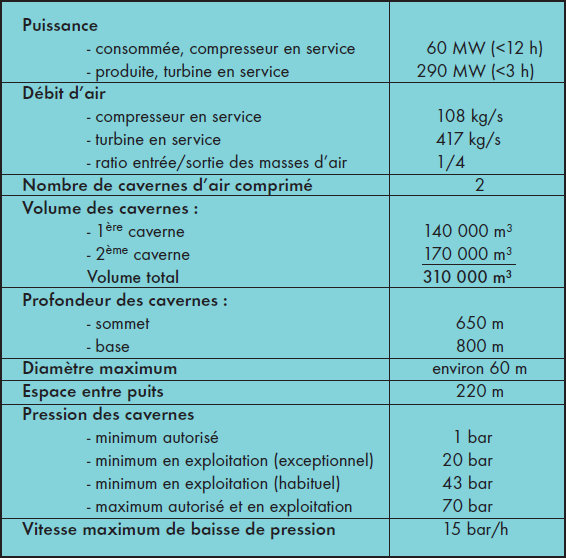
\includegraphics[scale=0.5]{PHOTO/tab1.png}
\label{tab1}
\end{figure}






\newpage

Puisqu'il nous manque un certain nombres de données, nous supposerons une compression avec un rendement isentropique de 80\%. L'air extérieur sera considéré comme étant à 300 Kelvin et à 1 Atmosphère. Nous considérons que la pression de sortie des compresseurs est de 70 Bar.\\

Nous calculons l'état de l'air après une compression isentropique. Cela nous permet d'écrire la formule suivante : 

\begin{equation}
Pr(T2)=Pr(T1)\frac{P2}{P1}
\label{pr_is}
\end{equation}

A l'état initial nous avons :

\begin{itemize}
\item T1=300K
\item P1=1atm
\item Pr(T1)=1,386
\item h1=300,19 kJ/kg\\
\end{itemize}

Donc à l'état final nous obtenons à partir de l'équation \ref{pr_is} et des tables de l'air :
 
\begin{itemize}
\item P2=70bar
\item Pr(T2)=97,0
\item h2=1000,55 kJ/kg
\item T2=960K\\

\end{itemize}

Avec un rendement isentropique ($\eta$) de 80\% nous avons l'équation \ref{rd_is}.

\begin{equation}
h3=\frac{h2-h1}{\eta}+h1
\label{rd_is}
\end{equation}

Ainsi, nous déterminons l'état "réel" 3 :

\begin{itemize}
\item h3=1175,64 kJ/kg
\item T3=1112,5 K\\

\end{itemize}



En sortie, les données nous disent que l'air à une température T4 de 310K. Ce qui nous donne une enthalpie h4 de 310,24 kJ/kg. De plus, on sait que le débit d'air est de 108 kg/s.
En considérant une transformation isobare et en appliquant le premier principe nous obtenons l'énergie récupérable :

\begin{equation}
Q=\dot{m}(h4-h3) = -93463.2 kW
\label{cha_recup}
\end{equation}


Nous regardons combien de kilogramme d'air sont stockées dans la caverne. L'objectif est de faire un bilan complet sur un cycle de stockage. 
Avec l'équation des gaz parfaits, nous obtenons la masse volumique de l'air à 70 bar et 310K (equation \ref{mv}). 

\begin{equation}
v4=\frac{P4}{T4*r}=80,00 kg/m^{3}
\label{mv}
\end{equation}

Avec $r=\frac{R}{M_{air}}=282,29 kg/m^{3}$\\


Nous faisons l'hypothèse que la température de l'air est constante pour une valeur de 310K.

Les cavernes de Huntorf ont un volume total de $310.000 m^{3}$. Nous pouvons donc stocker $2,48000.10^{7} kg$. Cependant, en pression, le minimum opérationnel des cavernes est de 43 bar. La masse volumique à cette pression est $v=49,14kg/m^{3}$. Donc on ne peut déstocker $1,52326.10^{7} kg$. Ce qui nous fait, au final, une masse utilisable de $m=0,95674.10^{7} kg$. \\

En reprenant le débit des compresseurs, nous remplissons la caverne en 92592 secondes. Nous obtenons donc pour un cycle de stockage $8,654.10^{9} kJ$ soit $2403,8 MWh$.\\
\newpage

\subsection{Calcule de la chaleur de combustion}

Nous allons estimer l'énergie nécessaire par combustion.

En entrée, nous avons un fluide qui arrive à 43 bar et 570K (état 5). Il est ensuite réchauffé à 803K dans une chambre de combustion (état 6). Nous regardons qu'elle est l'énergie qu'on a dû lui fournir pour une transformation isobare. \\


Nous avons donc :

\begin{itemize}
\item T5=570K
\item h5=575,59kJ/kg\\

\item T6=803K
\item P6=43bar
\item h6=825,25kJ/kg\\

\end{itemize}

Soit $Q_{combustion,1}=m(h6-h5)=663,5MWh$\\


Le passage dans la turbine provoque une détente qui fait passer le gaz à l'état 7 pour ensuite être réchauffé par une nouvelle combustion qui fait passer l'air à l'état 8.

\begin{itemize}
\item T7=650K
\item h7=659,84kJ/kg\\

\item T8=1140K
\item h8=1207,57kJ/kg\\

\end{itemize}

Soit $Q_{combustion,2}=m(h8-h7)=1455.6MWh$\\


Ce qui nous fait le total d'énergie de combustion nécessaire suivant :

 $Q_{total}=Q_{combustion,1}+Q_{combustion,2}=2118,5MWh$.\\

Au final, Nous pouvons remarquer que l'énergie perdue lors de la compression est supérieur à l'énergie nécessaire lors des combustions. Donc dans l'absolue, nous pouvons penser que si nous arrivons à stocker cette énergie de compression, nous pouvons supprimer l'utilisation de gaz naturel.\\

 Cependant, le manque d'information sur le système et en particulier sur le rendement des compresseurs ne permet pas d'avoir une quantification exacte de la réalité. Ce calcule nous donne seulement un ordre de grandeur mais permet tout de même de vérifier la pertinence de dimensionner un stockage de chaleur. De plus, la présence de gaz à très haute température permet de chauffer notre stockage de chaleur sensible aux alentours de 1000 Kelvin; ce qui permet par la suite de monter la température de notre air à celle souhaité tout en respectant le second principe.


\section{Analyse économique}

En France, le tarif réglementé du gaz naturelle s'élève à 0,0580 \euro TTC/kWh. Donc si nous occultons les rendements de la combustion, nous avons un coût en gaz naturelle de 122.873 euros pour un cycle de stockage. Si nous estimons un cycle par jour, nous avons un coût annuelle de 44.234.280 euros. Si nous imaginons que le stockage permet d'économiser 25\% de gaz naturelle, nous avons une économie annuelle de 11.058.570 euros. Supposons que l'on souhaite amortir l'investissement du stockage en 3ans, nous avons 33.175.710 euros disponible pour le réaliser. \\

En conclusion, nous pouvons clairement affirmer que ce stockage permet de réaliser un gain substantif rapidement.













\chapter{Présentation du code de dimensionnement}

\section{Introduction}

L'objectif du code est de dimensionner la taille du stockage sensible. Pour faire cela, il nous faut fixer une largeur et profondeur, la température de l'air que l'on souhaite en sortie, puis le programme calculera la hauteur de l'échangeur. 

Pour qu'il le réalise, nous avons discrétisé notre problème et rentré les équations de la chaleur. De ce fait, il calcule la température de l'air au cours du temps et analysera sa température final en sortie. Si elle est supérieure à celle souhaité, il rajoutera un certain nombre de tubes sur la hauteur et recommencera jusqu'à atteindre la consigne voulu.

Le concept général étant vus, nous allons maintenant le décrire en détaille. Nous verrons son organigramme, les hypothèses que nous avons dû faire, les équations que nous avons écrit, les variables d'entrées et de sorties.


\section{Hypothèse simplificatrice}

	Nous allons présenter dans cette partie les hypothèses faites pour coder notre modèle afin que les résultats obtenue soit bon tout en gardant un code relativement simple.\\
	
	Premièrement, la turbulence a été négligé. La rencontre du fluide avec des tubes cylindriques parallèle à l'écoulement provoque en effet de forte turbulence. Cependant, cela permet de favoriser l'homogénéisation de la température dans l'air. Nous pouvons donc tourner cela à notre avantage puisque sa nous permet de représenter une seul maille d'air entre deux tube de Cofalite. En contre partie, elle augmente aussi les pertes de charge dans l'échangeur. \\
	
	
	Cependant, nous allons faire une deuxième hypothèse en négligeant ces pertes de charge qui conduise à un baisse de pression mais de manière assez négligeable.  \textcolor{red}{Faire un ptit truc EES pour vérifier que cela est vrai. il parait qu'il y a une petite formule dans le truc de bédécarrat ou l'on a trouvé la corrélation de H} 
	
	Pour finir, nous négligeons également les transferts par rayonnement. Même si nous avons des températures assez élevées, la complexité pour intégrer les équations de rayonnement dans ce code est très importante. Nous ne connaissons pas les facteurs de forme qu'il y a entre les tubes et nous devrions calculer l'absorptivité de l'air en fonction de la pression et température.

	Ces hypothèses nous ont menées au maillage décrit dans la section qui suit.




\newpage
\section{Le maillage}

Nous avons discrétisé en espace un élément de notre échangeur puis nous avons répété ce schéma sur la hauteur. Nous avons donc une hauteur d'échangeur qui est : hauteur = diamètre du Cofalite $\times$ nombre de tubes.

Nous avons discrétisé en volume constant le tube le Cofalite (voir le schéma \ref{maillage}) \\


Nous présentons ci-dessous les schémas avec les grandeurs caractéristiques :




\begin{figure}[!h]
\centering
\caption{Configuration Géométrique}
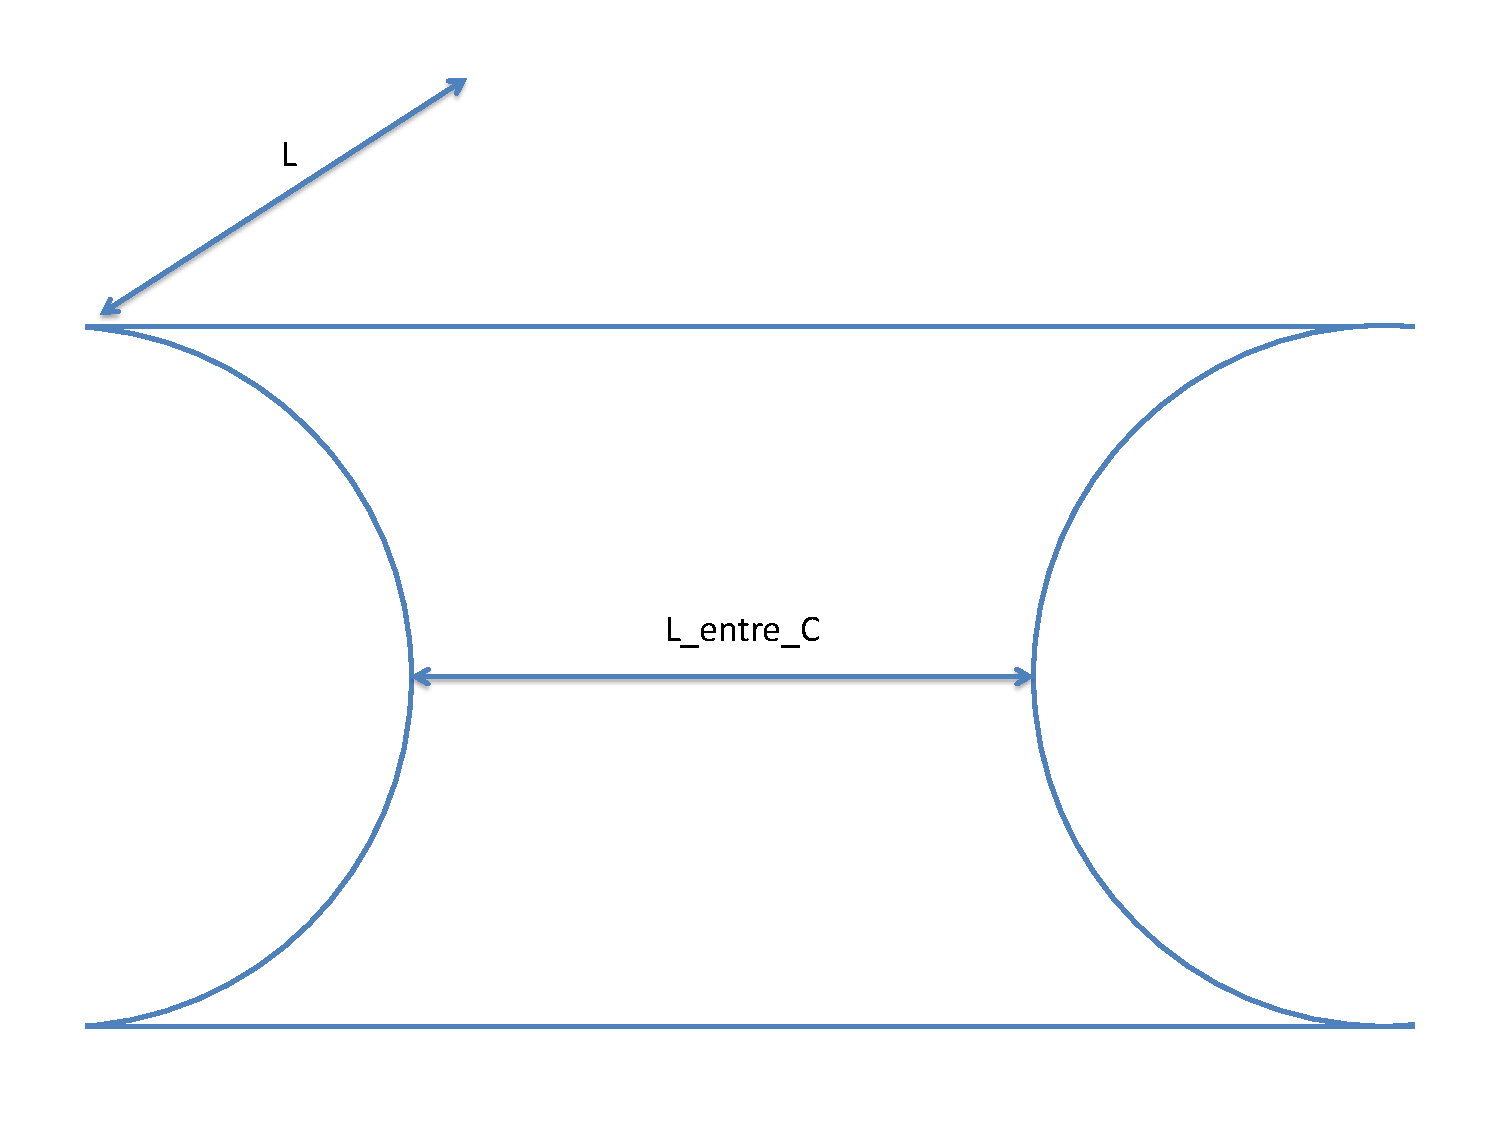
\includegraphics[scale=0.35]{PHOTO/Shema_conf_geo.pdf}
\label{conf_geo}
\end{figure}



\begin{figure}[!h]
\centering
\caption{Maillage}
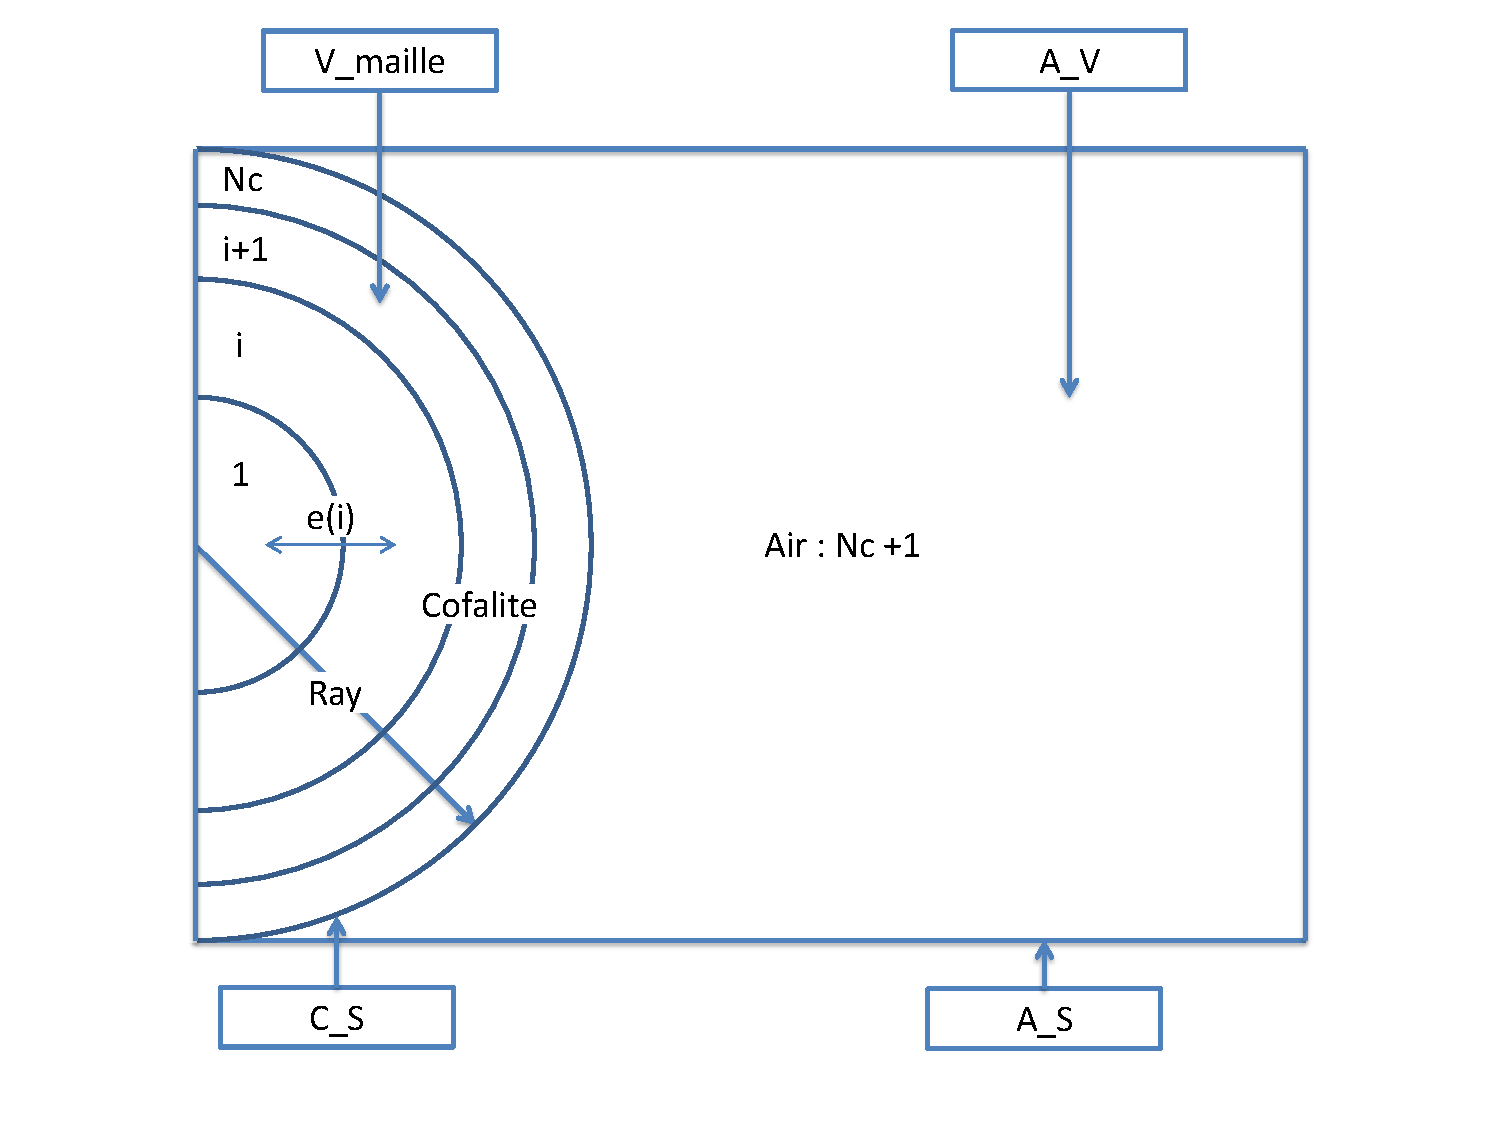
\includegraphics[scale=0.5]{PHOTO/Shema_maillage.pdf}
\label{maillage}
\end{figure}



\newpage


\section{Équations physiques résolues}
\textcolor{red}{LES ECRIRES}


\section{Variables d'entrées et de sorties}

	\subsection{Variables d'entrées}
	
		\subsubsection{Géométriques}
		
		Nous avons laissé, à l'utilisateur, une certaine marge de manœuvre pour adapter l'échangeur. 
		Ainsi, il peut fixer le rayon de chaque tubes de Cofalite. C'est la variable "Ray". 
		Il peut fixer la distance entre deux tubes sur le plan horizontale. C'est la variable "L\_entre\_C".
		
		Nous avons considéré que les contraintes d'espace sont plus déterminante au niveau de la surface au sol et moins sur le plan de la hauteur. De ce fait, l'utilisateur doit rentrer ses conditions sur la largeur et la profondeur de l'échangeur. Comme nous ne pouvons pas prédéterminer la hauteur de notre stockage il est fortement possible que celle-ci soit très importante. Par conséquent, ci celle ci ne lui convient pas, il devra soit augmenter la surface au sol, soit diminuer la température de consigne.\textcolor{red}{ Nous avons cependant rajouter une variable d'entrée intitulé "Hauteur\_max" qui permet de stopper de le code en cas de dépassement et donner un message d'erreur à l'utilisateur.}
		La variable de la profondeur s'intitule "L"; celle de la largeur "largeur".
		
		
		\subsubsection{Physique}
		
		Pour le stockage, nous devons mettre en place trois échangeurs (un entre chaque compresseur). De ce fait, L'air sort à une pression et température différente. 
		
		Nous avons fixer la pression pour trois valeurs différentes qui sont celle indiquer sur le schéma \ref{sh_fonc}, c'est à dire 4, 27 et 70 bar. L'utilisateur devra donc en indiquer une. Celle-ci permettra de considérer les propriétés de l'air à celle ci en fonction de la température.
		\textcolor{red}{ il faut faire le destockage à 50 bar!!!!!}\\
		
				
		Pour ce qui est de la température, l'on doit fixer la valeur de l'air. C'est la variable nommé "T\_entree". Nous avons fait un petit programme EES qui permet de les calculer. Il suffit de régler le rendement isentropique et \textcolor{red}{la température de sortie de l'air après passage dans les échangeurs.}
		Il faut également donner la température initiale de Cofalite (autour de 298K qui est la température de l'air à l'extérieur)
		
		\textcolor{red}{Pour le destockage, nous lirons la température du Cofalite après le stockage avec un éventuelle temps d'attente entre le stockage et destockage. En effet, la conductivité de celui ci est de $2 W.m^{-1}.K^{-1}$ et par conséquent, il existe un gradient de température au sein même du matériau.}\\
		
		Nous indiquerons aussi le débit d'entrée du Cofalite dans l'échangeur. Pour le stockage les données nous indique du $108kg.s^{-1}$, tendis que pour le destockage nous avons du $417kg.s^{-1}$ (voir tableau \ref{tab1}). 
		
		\subsubsection{Discrétisation}
			\paragraph{En espace :}
			
		L'utilisateur peut régler le nombre de maille sur le Cofalite avec la variable "Nc". Augmenter ce nombre rajoute de la précision sur le gradient de température au sein du matériau mais, de ce fait, améliore également la précision sur la température de sortie de l'air. Cependant, le temps de calcule augmente grandement. C'est pourquoi nous laissons l'utilisateur choisir en fonction de ses préférences. Attention, Nc doit avoir une valeur minimal de 3 pour que le code converge.
			\paragraph{En temps :}
		L'utilisateur fixe le temps de l'expérience, variable intitulé "T\_max". Pour le stockage nous avons un temps au alentour de $9\sim12$ heures (Heures creuses) et un temps de destockage de 3 heures (Heures pleines). 
		
		Nous indiquons le pas de temps. Le programme est assez robuste donc il peut être assez élevé, mais attention, cela reste du semi-implicite. \textcolor{red}{Une analyse de sensibilité sera faite plus loin}.
		
		
			  
\section{Organigramme}
	Nous présentons ici les organigrammes qui expliquent le fonctionnement de notre code.\\
	
	\textcolor{red}{ (à compléter/modifier)}
	Ci-dessous le fonctionnement de la principale subroutine "element" qui permet de résoudre le système pour chaque pas de temps.
	
\begin{figure}[!h]
	\centering
	\caption{Organigramme de la subroutine "element"}
	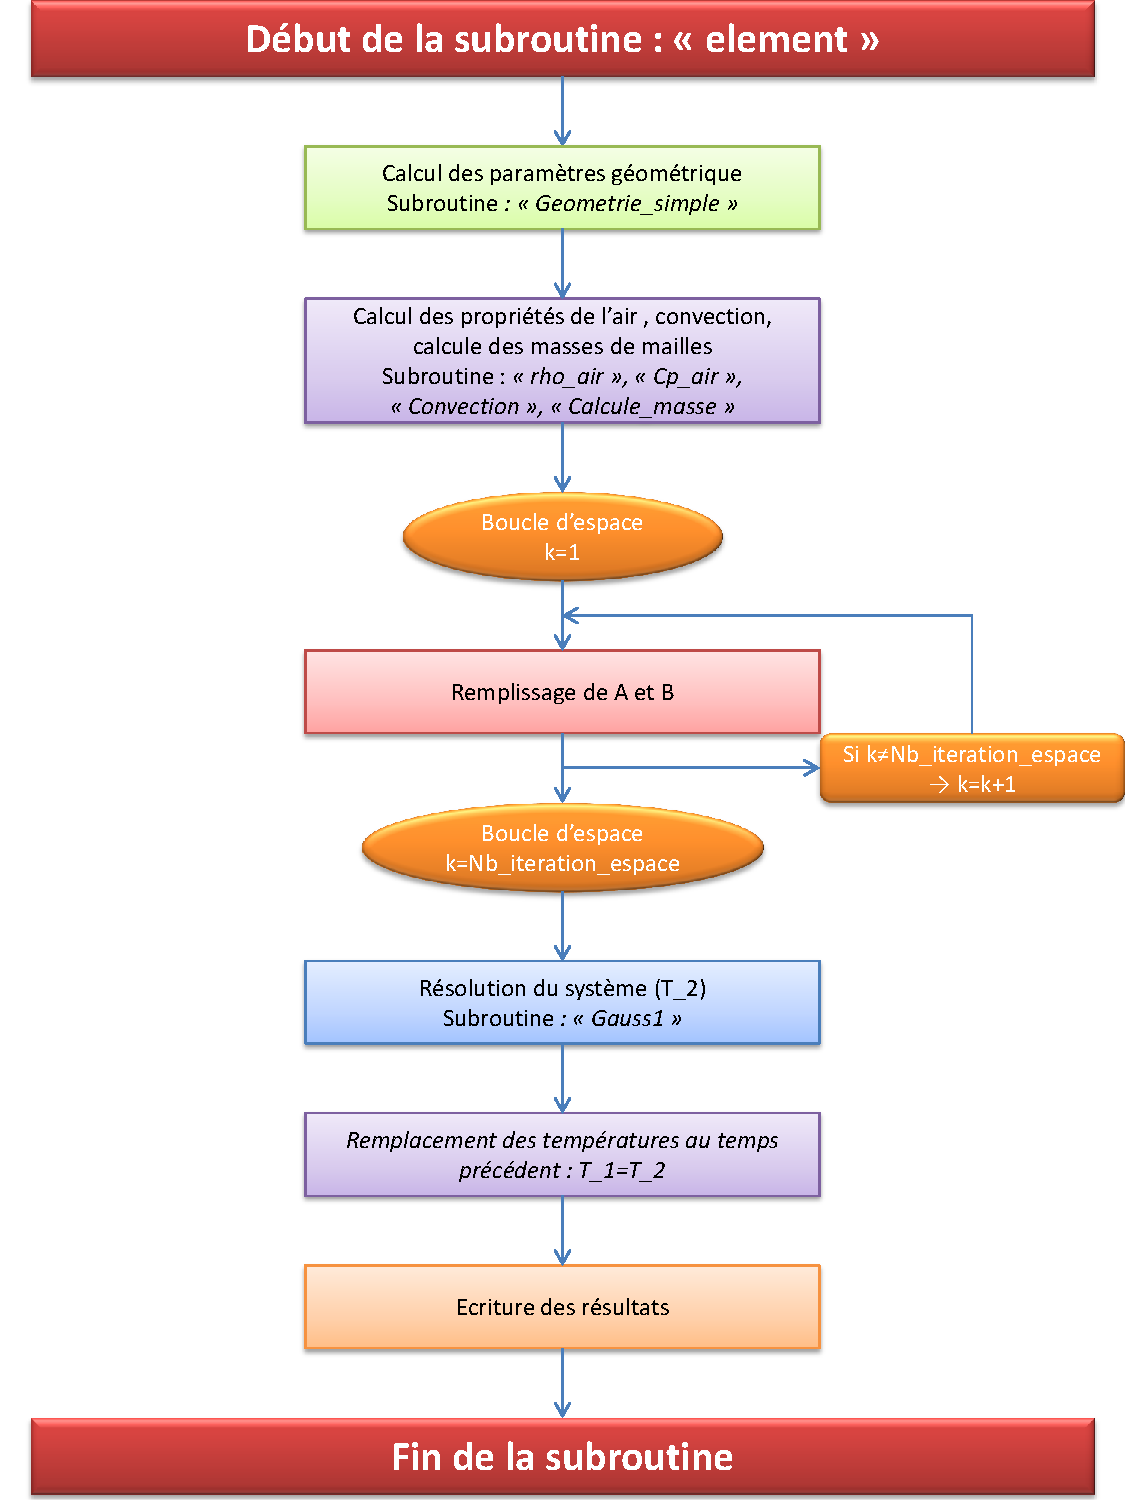
\includegraphics[scale=0.75]{PHOTO/Organigramme_element.pdf}
	\label{orgasme_element}
\end{figure}
	
		
	\newpage
	
	
		
		
\section{Vérification du code}		
		
Plusieurs simulations peuvent témoigner de la validité du code.

\subsection{Convergence}
		
Afin de tester la convergence des résultats, il convient de tester la convergence de la température du cofalit avec un temps de simulation suffisamment long.
Ainsi, le temps de simulation a été fixé à $1.10^{7}s$ avec un pas de temps de 10 secondes, pour une température d'air en entrée de 570K, et une température initiale de cofalit de 298K.
Le nombre de tube sur la hauteur a été fixé a 20 afin que le temps de simulation soit réduit au minimum.
Ainsi, les résultats affiché donne une température du cofalit a 570K quelque soit la maille considérée. La convergence du code est donc bien justifiée ici.

\subsection{Coherence du code}

Afin de vérifier la cohérence du code, la température de l'air en entrée a été fixé à la même valeur que celle du cofalit initialement.
Ainsi, quelque soit le temps de simulation, la température de l'air et du cofalit ne doit pas varier, et le transfert de chaleur doit être nul. 
Cependant, après simulation, la valeur du flux est de $8,7.10^{-6}J$, pour un temps de simulation de 100s, et avec 20 tubes de cofalit en hauteur.


\chapter{Optimisation du dé-stockage}

\section{Problème rencontré}

Les premiers résultats du dé-stockage obtenues sont présentés ci-dessous.


\textcolor{red}{mettre les résultats obtenus}


Nous pouvons remarquer que lors du dé-stockage notre énergie récupéré est faible comparé à ce qui a été stocké. Nous devons par conséquent trouver des façons de l'améliorer. \\

La première idée serait d'augmenter le nombre de tube pour augmenter les surfaces d'échanges. Cependant, si l'on augmente le nombre de tube, les derniers tubes vont avoir une température relativement faible. De ce fait, lors du dé-stockage, l'air ne va quasiment pas se réchauffer sur les tubes rajoutés. Ce n'est donc pas une solution approprié. \\

Nous allons mettre en avant un point important. Sur notre premier stockage, la température initiale des tubes est celle de la température atmosphérique. Mais lorsque l'on dé-stocke, l'énergie n'étant pas totalement récupéré, la température initiale des tubes, pour le prochain stockage, ne va plus être la même. De ce fait, il va s'instaurer un régime d'équilibre au cours de quelques stockages.\\

Si l'on stocke toujours de la même manière, nous allons avoir un profil de température suivant au cour des stockages. 

\begin{figure}[!h]
	\centering
	\caption{Cycle 1 : Profil de température dans l'échangeur}
	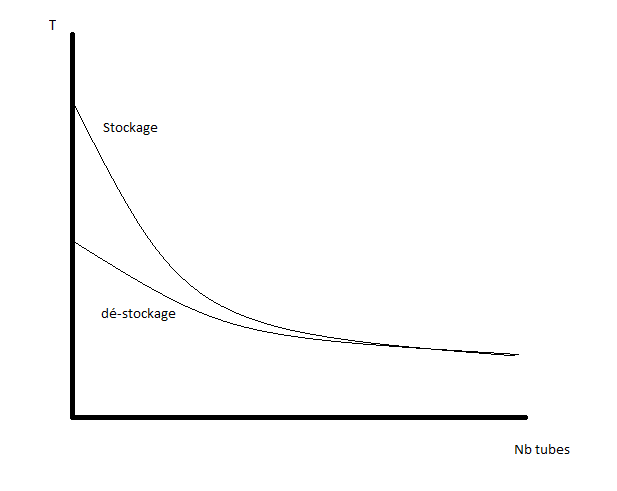
\includegraphics[scale=0.4]{PHOTO/courbe1.png}
	\label{graph1}
\end{figure}

\begin{figure}[!h]
	\centering
	\caption{Cycle 2 : Profil de température dans l'échangeur}
	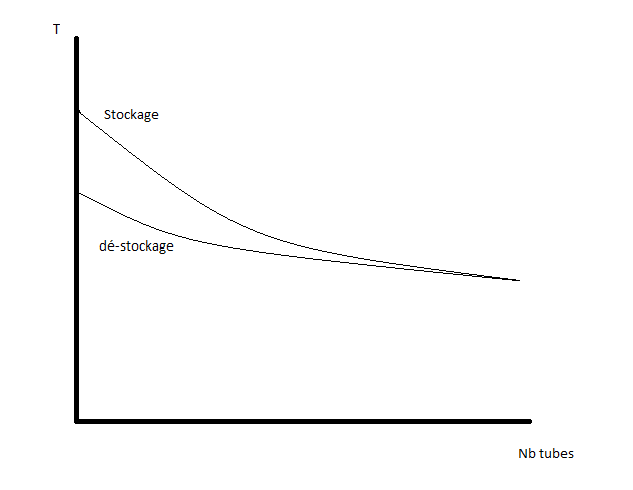
\includegraphics[scale=0.4]{PHOTO/courbe2.png}
	\label{graph2}
\end{figure}

\begin{figure}[!h]
	\centering
	\caption{Cycle nominal : Profil de température dans l'échangeur}
	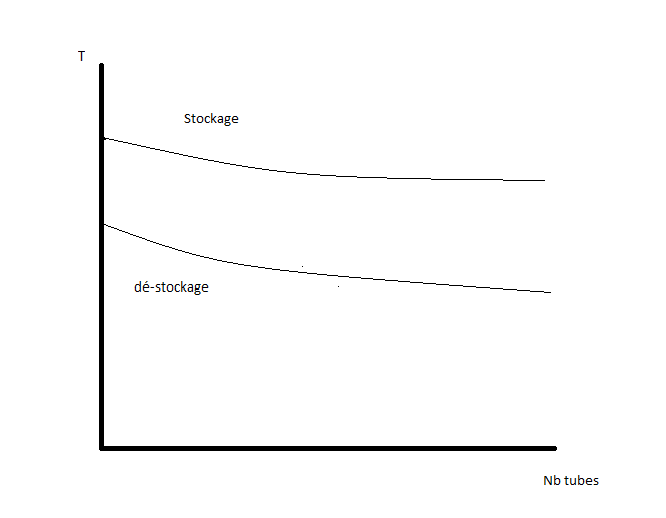
\includegraphics[scale=0.4]{PHOTO/courbe3.png}
	\label{graph3}
\end{figure}

\newpage

 Ce qui est essentiel de comprendre dans ces graphiques, c'est que nous avons un régime nominal qui se met en place au cour des stockages. Par conséquent, notre dimensionnement doit être fait pour le régime nominal. Ce qui va nous conduire à crée une boucle supplémentaire qui sera décrit dans le paragraphe suivant. 
\newpage

Nous pouvons remarquer qu'en alternant le sens de l'air dans le stockage de chaleur, nous avons une mise en place et un profil de régime nominal différent. Si on alternait le sens de l'air sur chaque cycle de stockage, le profil de température obtenue aurait l'allure suivante : 


\begin{figure}[!h]
	\centering
	\caption{Cycle nominal : Profil de température dans l'échangeur avec alternance du sens de l'air}
	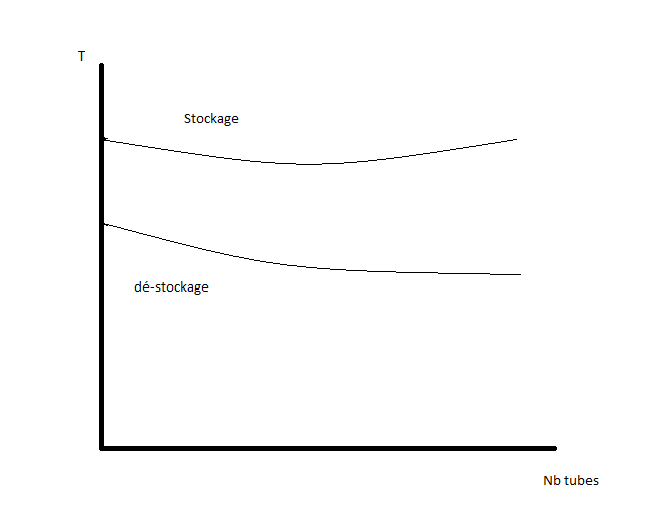
\includegraphics[scale=0.4]{PHOTO/courbe4.png}
	\label{graph4}
\end{figure}

Nous pourrions alors rechercher la meilleur configuration en alternant le sens du stockage et de-stockage. Nous nous limiterons ici au premier cas. 

\newpage
\section{Organigramme de la boucle}

\begin{figure}[!h]
	\centering
	\caption{Organigramme du dimensionnement en régime nominal}
	\includegraphics[scale=0.75]{PHOTO/organigramme_final.pdf}
	\label{graph3}
\end{figure}

\newpage

\include{sol_alternative}
\section{Nouveau Programme}

\subsection{Introduction}

Le nouveau programme, réalisé tardivement, accélères énormément les temps de calculs. Une simulation réalisé avec l'ancien programme à mit plus d'une heure alors que celle lancé avec le nouveau a durée que quelques secondes.

Grâce à cela, il nous est maintenant possible de dimensionner une installation beaucoup plus importante est plus cohérente. En effet, nous pouvons maintenant modéliser l'évolution de la température à travers de nombreux tubes et donc imaginer un serpentin avec une section d'entrée faible, conditionné sous forme d'un cube.

\subsection{Principe logique}

Le problème étant la taille de la matrice de résolution, nous avons segmenté sa taille. Nous résolvons l'équation pour un nombre d'élément définit par la variable $"Nb\_iteration\_espace"$.

 Ainsi, si nous mettons un élément, nous calculons ses températures en résolvants une matrice carré de taille Nc+1. Pour faire cela, nous faisons le calcule pour un élément, nous écrivons le résultat et nous stockons les températures dans une matrice. 
 
 Après avoir réalisé cela sur le stockage et de-stockage, nous passons à un autre élément en récupérant les valeurs de la résolution précédente. Ainsi, nous complétons l'échangeur au lieu de tous recalculer avec une énorme matrice. Nous devons bien noté que nous stockons la température de l'air de sortie de l'élément à tous les pas de temps, dans un vecteur, car l'élément suivant est essentiellement dépendant de la température de l'air de l'élément précédant à tous les pas de temps. 

Pour clarifier cette explication nous présentons l'organigramme dans la section qui suit.

\newpage
\subsection{Organigramme}

\begin{figure}[!h]
\centering
\caption{Organigramme du nouveau programme : partie 1}
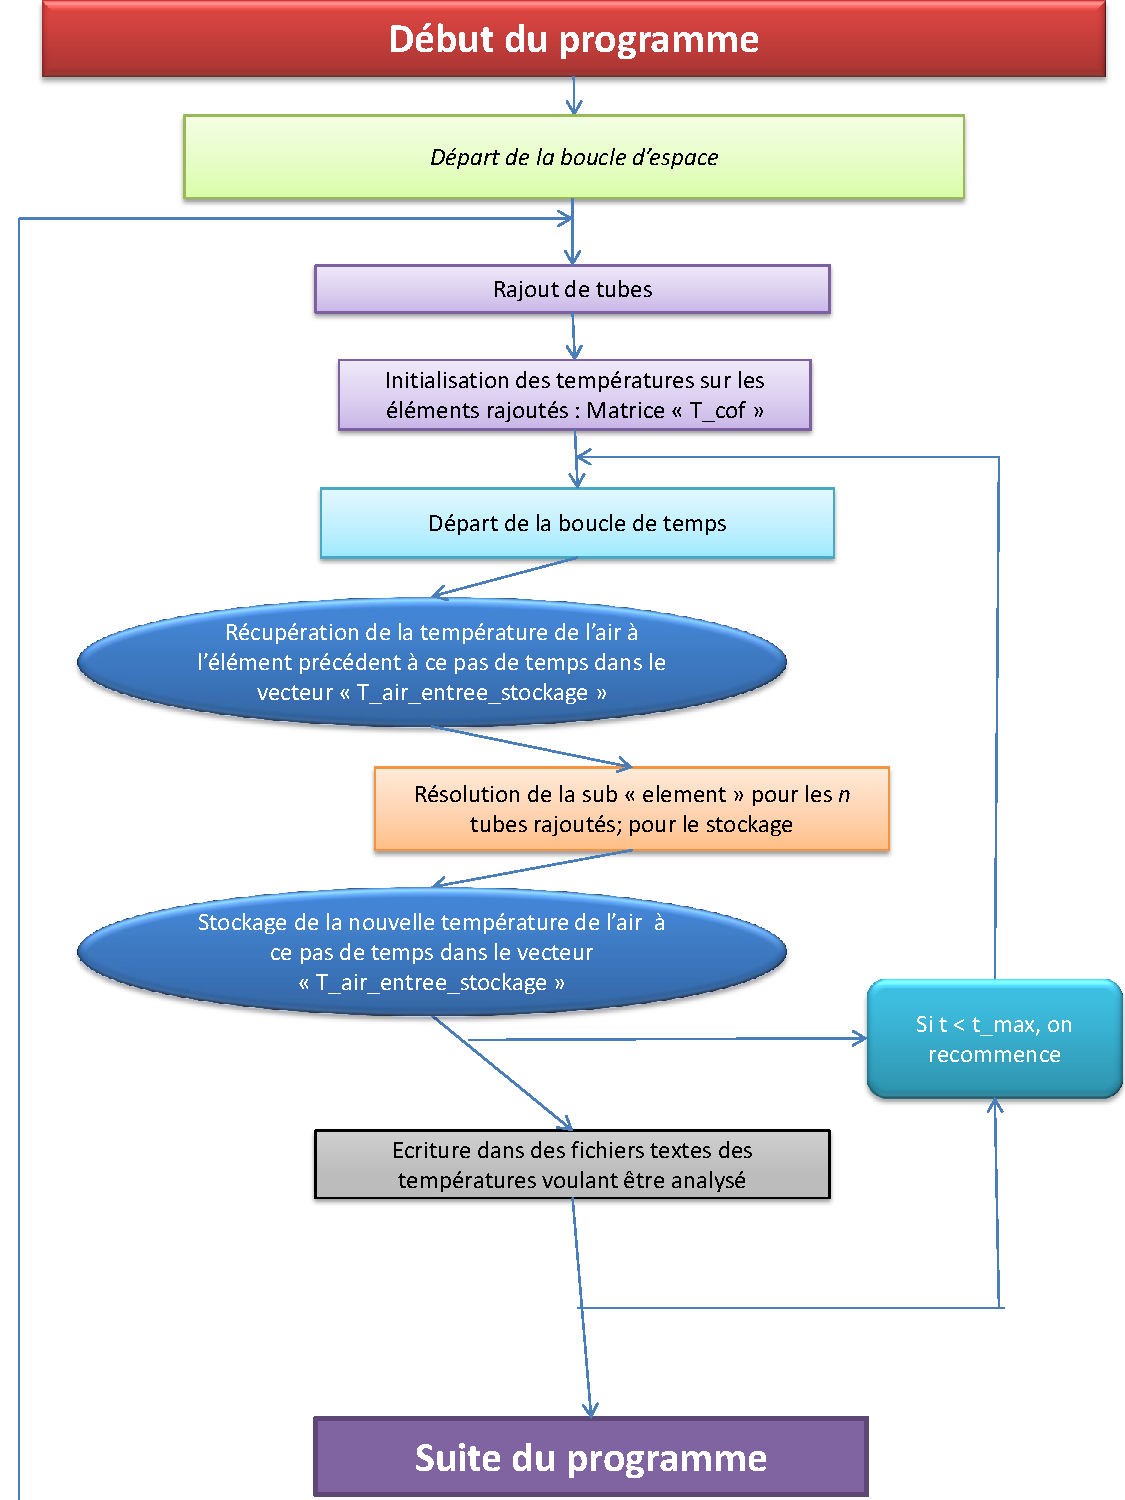
\includegraphics[scale=0.8]{PHOTO/Organigramme_dernier_prog_1.pdf}
\label{dernier_prog_1}
\end{figure}



\begin{figure}[!h]
\centering

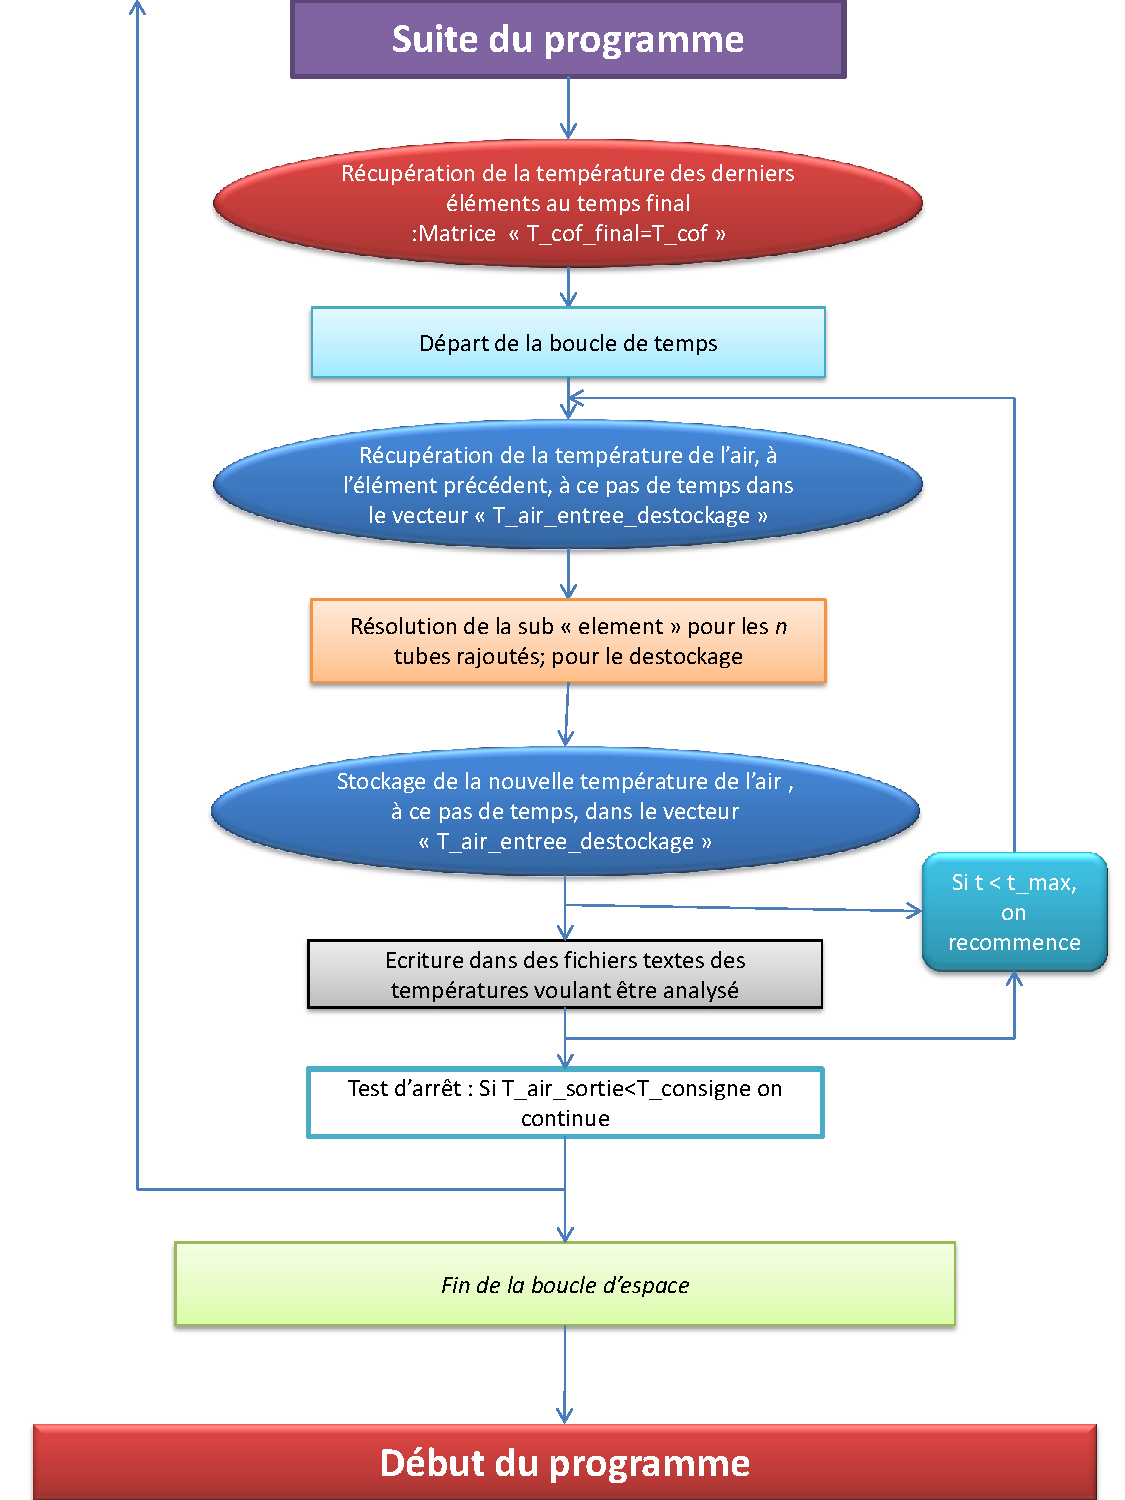
\includegraphics[scale=0.8]{PHOTO/Organigramme_dernier_prog_2.pdf}
\label{dernier_prog_2}
\caption{Organigramme du nouveau programme : partie 2}
\end{figure}
\clearpage




\subsection{Critère d'arrêt}

Nous avons uniquement deux tests d'arrêts sur la version actuelle. L'un permet d'arrêter les itérations sur l'espace lorsque l'on atteint la Température de consigne lors du déstockage. Le deuxième est indirect. La boucle qui rajoute les tubes stop lorsque l'on atteint la valeur de la variable $"Nb\_boucle\_rajout\_tube"$, fixé par l'utilisateur. Nous remarquons indirectement que la multiplication du nombre de tube rajouté, sur chaque pas de la boucle, avec l'indice du pas, donne le nombre de tube sur la hauteur.

Nous fixons donc le nombre de tube par la formule suivante :

\begin{equation}
Nb_tubes=Nb\_boucle\_rajout\_tube * Nb\_iteration\_espace
\end{equation}

\subsection{Remarque}

La variable $"Nb\_iteration\_espace"$ doit être la plus petit possible pour accéléré la vitesse de calcul. Aucun bug notable a été remarqué pour une valeur de 1 et donc ce nombre est conseillé. \\
 
Les tailles de matrice sont les suivantes : 
\begin{itemize}
\item $T\_cof = (Nc+1)Nb\_iteration\_espace$
\item $T\_cof\_final = (Nc+1)Nb\_iteration\_espace$
\item $T\_air\_entree\_stockage = Nb\_iteration\_temps$
\item $T\_air\_entree\_destockage = Nb\_iteration\_temps$
\item Matrice de résolution A : $A = ((Nc+1)Nb\_iteration\_espace) \times ((Nc+1)Nb\_iteration\_espace)$\\

\end{itemize}


Cette astuce pour accéléré drastique-ment la vitesse de calcule numérique a été pensé et réalisé la veille de la date butoir. 
Ainsi, nous n'avons pas eu le temps nécessaire pour perfectionner les détailles et lancer une simulation pour un installation réelle. Cependant, la version actuelle reste fonctionnel et nous présenterons les nouveaux résultats obtenus lors de la soutenance oral.




\chapter*{Conclusion}
\addcontentsline{toc}{chapter}{\protect\numberline{}Conclusion}



Ce projet a permit de réaliser un programme permettant le dimensionnement d'une unité de stockage sensible en régime in-stationnaire. Nous avons rencontré énormément de problèmes numériques pour réaliser ce dernier. De ce fait, nous avons dut nous contenter de simulations pour de petites dimensions. Grâce à ces dernières, nous avons fait de nombreuses analyses de sensibilités permettant de mettre en avant les subtilités de ce type de stockage.\\

Le projet avait pour objectif de dimensionner une unité de stockage pour la central de Huntorf. De ce fait, nous avons fait des calculs préliminaires pour constater l'avantage de récupérer la chaleur des compresseurs sur ce type d'installation. De plus, nous avons évalué un ordre de grandeur de l'investissement possible pour installer notre système. Nous avons par la suite estimé la température en sortie des compresseurs pour connaitre les caractéristiques de l'air en entrée de notre échangeur. Ainsi, nous avons posé les données essentielles à notre simulation. Cependant, la complexité du programme nous a empêché de la réalisée, puisque les dimensions nécessaire étaient trop grande, même pour le cas idéal. Ceci dit, la récente amélioration du programme devrait permettre de faire cela. Nous ferons en sorte de vous présenter les résultats lors de la soutenance oral. Un petit sursis de temps nous aurait également permit de lui attribuer les quelques astuces programmé dans sa version précédente, mais surtout les calculs pour le dimensionnement en régime régime nominal. Bien que l'objectif n'a pas été parfaitement accomplit, il faut tout de même noter que nous avons écrit des programmes de plus de milles lignes et que nous avons fini par aboutir sur une version très puissante (donc très rapide). De plus, il peut très bien être utilisé pour simuler n'importe qu'elle type d'échangeur, de même configuration, en régime in-stationnaire. Réalisé ce que nous avons fait dans un laps de temps aussi serré était loin d'être facile et par conséquent nous somme amplement satisfait de ce que nous avons accomplit. 





\end{document}